% $Id: AllegProposal.tex,v 1.8 2000/07/05 21:02:12 culver Exp $
% AllegProposal.tex
% by A. Thall
% 13. Feb 2003
%
% Small edits and a few additions made by R. Roos
% 21 Jan 2007
% Most particularly, the "box" around the thesis statement has been removed,
% section titles have been modified. The section named "Prior work II" has
% been commented out. The \topmargin has been changed to -.5in and the
% change to \parindent has been commented out.
% The filename "nausicaa.eps" has been changed to simply "nausicaa" so that
% pdflatex can be used on the file (and a file named "nausicaa.pdf" has
% been created using the "epstopdf" command).
% Several subsections have been added to illustrate subsection usage.
% The word "comp" has been replaced by "project" or "thesis" throughout.
% Other small changes have been made.
%
% This document provides a sample Senior Project Proposal template for use
% by students in Allegheny's CS and Applied Computing programs.

\NeedsTeXFormat{LaTeX2e}
\documentclass[11pt]{article}
\usepackage[utf8]{inputenc}
%The following is used by WinEdt to set up cross-referencing to the BibTeX files
%It is NOT commented out---the comment lets it be simply ignored by non-WinEdt LaTeX compilers

%GATHER{mybibtexDB.bib}

\usepackage{setspace}
\usepackage{amsmath}
\usepackage{amssymb}
\usepackage{epsfig}
\usepackage{fancybox}
\usepackage{listings}
\usepackage{algo}
\usepackage{url}

\setlength{\textheight}{9in}
\setlength{\textwidth}{6in}
\setlength{\oddsidemargin}{.25in}
\setlength{\topmargin}{-.5in}  % changed from -.25 by RSR on 1/21/07
%\parindent .5in    % commented out by RSR 1/21/07

%put words in the hyphenation statement if you want to enforce
%how LaTeX should break them (or not) at the end of a line.
%\hyphenation{repre-sen-tations problems exact linear}
\hyphenation{itself}

%%%%%
%% Commented out -- RSR, 1/21/07
%%%%%
% The following provides a box to surround the thesis statement
%\newenvironment{Thesis}%
%{\begin{Sbox}\begin{minipage}{.95\linewidth}}%
%{\end{minipage}\end{Sbox}\begin{center}\fbox{\TheSbox}\end{center}}

\title{Relatório Parcial: Ano 2}
\author{Isaac L.\ Santos\ Sacramento \\ Orientador: Mauro Roisenberg}

\begin{document}

% You can specify a language and other options for
% the code-formatting "listings" package
\lstset{language=C++,basicstyle=\small,
        stringstyle=\ttfamily,showstringspaces=false}

\singlespace
\maketitle

\begin{abstract}                % ~350 words max
Neste relatório são apresentadas as atividades realizadas no segundo ano de projeto, mais precisamente no
período de março a outubro de 2016. Neste período foram realizados estudos e experimentos relacionados à aplicação
de \textit{Deep Learning} para realizar simulação geoestatística multiponto. Estas atividades estão descritas
nas seções a seguir.

\end{abstract}

\doublespace
% This sets section-numbering to only include Section and Subsection numbers
\setcounter{secnumdepth}{2}

\section{Introdução}

No período de março a outubro de 2016 foram exploradas duas novas frentes de trabalho relacionados ao estudo da incerteza.
Inicialmente, foram estudados os algoritmos de simulação multiponto, por meio dos quais é possível
gerar realizações de fenômenos geoestatísticos condicionadas a amostras reais disponíveis. A simulação multiponto utiliza
imagens de treinamento como dados de entrada para definir a estrutura espacial de um processo \cite{Guardiano1993} e difere
dos métodos baseado em variograma, pois utilizam um conjunto de pontos na vizinhança do ponto simulado.
As imagens de treinamento são descrições explícitas, 2D ou 3D, da continuidade espacial estudada e, a partir delas,
podem ser extraídas estatísticas de múltiplos pontos, inclusive o variograma.
Em particular, o algoritmo FILTERSIM despertou o interesse na utilização de técnicas de \textit{Deep Learning}
para realização de simulação geoestatística devido a sua similaridade com a definição de Redes Neurais Convolucionais. O algoritmo é descrito
com maior detalhe na seção seguinte, juntamente com outros algoritmos de simulação geoestatística multiponto.

A etapa do trabalho está relacionada à utilização de técnicas de \textit{Deep Learning} e seu potência de aplicação para solução de
problemas relacionados a simulação geoestatística. Foram realizados estudos para a definição de um método capaz de realizar
simulação multiponto utilizando o conceito de \textit{Deep Learning}. As redes neurais convolucionais (RNC) estão no centro
das pesquisas relacionadas a aprendizagem de máquina. As RNC são muito populares nas áreas de classificação de imagens \cite{Krizhevsky2012,He2014},
visão computacional \cite{Zhangg_2014}, reconhecimento de faces \cite{NyiSun2014}, à segmentação de imagem e reconhecimento de ações em vídeos;
Os fatores que conferem às RNC a importância atual são: (i) a eficiência no treinamento em GPUs modernas, (ii) a proposta das Unidades Lineares Retificadas
(em tradução livre do termo em inglês Rectified Linear Unit - ReLU)  as quais tornam a convergência mais rápida,
e (iii) o acesso amplo aos dados para treinamento de modelos extensos (ImageNet)\cite{Krizhevsky2012}.
Semelhante aos algoritmos de simulação geoestatística multiponto, as redes neurais convolucionais utilizam imagens de treinamento como dados de entrada.
Como visto anteriormente, as RNC são amplamente utilizadas para resolver problemas de classificação. Entretanto, visando realizar simulações
geoestatísticas, experimentos são realizados com diferentes conjuntos de dados a fim de obter um modelo regressivo de redes convolucionais.


\section{Revisão Bibliográfica}

Os métodos tradicionais de simulação se apoiam na modelagem de estatísticas em dois pontos, geralmente as covariâncias e variogramas. Muitos
fenômenos são complexos e inviabilizam a captura de seus padrões espaciais por meio de estatísticas de dois pontos. A simulação
geoestatística multiponto é um método genérico e se
baseia em três mudanças conceituais formalizadas por \cite{Guardiano1993}. A primeira, afirma que conjuntos de dados podem não ser suficiente
para inferir todas as características estatísticas que controlam o que se deseja modelar. A segunda é adotar uma estrutura estatística
não-paramétrica para representar a heterogeneidade. A terceira mudança conceitual é avaliar a estatística de eventos de dados de múltiplos
pontos. As estatísticas multipontos são expressas como funções densidades cumulativas para uma variável aleatória $Z(x)$ condicionadas
a eventos de dados locais $d_n =  {Z(x_1), Z(x_2),...,Z(x_n)}$, isto é, os valores de $Z$ nos nós vizinhos $x_i$ de $x$, equação \ref{eq:1}.
\begin{equation}
 f(z, x, d_n) = Prob({Z(x)<=z|x})
 \label{eq:1}
\end{equation}

Os diferentes algoritmos que compõem este método compartilham elementos comuns, como o uso de um caminho
de simulação (geralmente aleatório), a amostragem em distribuições de probabilidades locais e o uso de grades múltiplas \cite{Mariethoz2014_A}.
\cite{caers_1998} apresentam um modelo de simulação multiponto baseado em redes neurais que utilizam imagens de treinamento
como fonte de aprendizado. Deste modo, as redes neurais podem ser ensinadas a coletar estatísticas de múltiplos pontos e utilizá-las
para gerar modelos probabilísticos condicionados aos dados reais. Para realizar esta tarefa, as distribuições condicionais aprendidas
pela rede, relacionam o valor em qualquer região da imagem aos dados da sua vizinhança, dentro de um \emph{template} centrado na região
simulada, semelhante à ilustração da figura \ref{fig:templates}.
\begin{figure}[!htb]
   \centering
   \caption{Definição de uma vizinhança.}\label{fig:templates}
   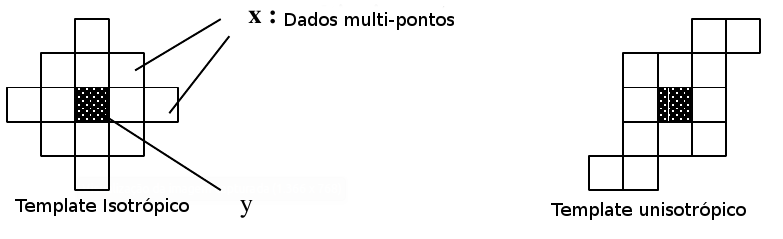
\includegraphics[width=0.6\textwidth]{figuras/templates.png} \\
   \small{Fonte: \cite{caers_1998}}
\end{figure}
A rede neural é treinada para determinar os valores de $y$ em qualquer região, dados os valores da vizinhança $x$. Matematicamente,
a rede neural modela a função densidade de probabilidade (FDP) local da equação \ref{eq:a}, ou sua integral, a função de distribuição condicional cumulativa (FDCC).
\begin{equation}
 f(y|x) = Pr({y<Y<y+dy|x})
 \label{eq:a}
\end{equation}

A abordagem multiponto baseada em redes neurais \cite{caers_1998}, fortaleceu o
interesse no estudo dos métodos multipontos. Em 2002, o algoritmo \emph{SNESIM} \cite{Strebelle2002_B} foi apresentado como uma alternativa
para realizar simulações sequenciais livres de variogramas e capazes de lidar com a presença de padrões não-estacionários
nas imagens de treinamento. Este algoritmo utiliza estrutura de árvore para armazenar a distribuição de probabilidade condicional
calculada a partir da imagem de treinamento. Em 2011, \cite{Straubhaar2011} apresentaram o método \emph{IMPALA}, 
que consiste na implementação do método multiponto original, com a substituição da árvore de busca por uma estrutura de lista.
Esta medida permite reduzir a quantidade de memória RAM utilizada pelo algoritmo e, consequentemente, utilizar diferentes
listas para guardar dados adicionais igualmente utilizados durante a simulação. 
Em 2010 o algoritmo \emph{simulated annealing} foi implementado com intuito de gerar realizações estocásticas de variáveis
categóricas por reprodução de estatísticas multipontos \cite{Peredo20111110}. A imagem de treinamento é
utilizada para determinar as frequências de ocorrência das configurações de cada nó. Estas frequências são
usadas como estatística alvo que deve combinar com as imagens estocásticas geradas com o algoritmo. 

Os algoritmos, \emph{SNESIM} e \emph{IMPALA}, se baseiam no armazenamento dos eventos de dados encontrados na imagem de treinamento, são restritos 
à simulação de variáveis categóricas e necessitam de um modelo para a vizinhança do ponto simulado. Uma nova abordagem para SMP procede com 
amostragens diretamente sobre a imagem de treinamento para um determinado evento, de modo que o uso de um banco de dados de evento se torna 
dispensável \cite{Mariethoz_2010} \cite{Meerschman_13}. O método de amostragem direta permite estender a aplicação de geoestatística multiponto para variáveis contínuas 
e categóricas e se destaca por respeitar a distribuição de probabilidade condicional sem realizar a sua computação. Na utilização de múltiplas 
variáveis, uma função $d$ é escolhida apropriadamente para variáveis categóricas ou contínuas. É possível utilizar a função de distância ($d(.)$) 
para controlar as proporções globais e locais, ou impor uma média local. Para tanto, é adicionado um fator de erro ($E_p$) à fdp, que quantifica a 
diferença entre a probabilidade alvo $L(x)$ e a proporção atual $P\*(x)$ na grade $SG$ parcialmente simulada, na forma da equação \ref{eq:b}.
\begin{equation}
 E_p ~ |P\*(x) - L(x)|
\label{eq:b}
\end{equation}

Uma observação comum na comparação entre a imagem de treinamento e as realizações geradas é a existência de padrões exatamente reproduzidos da imagem de treinamento para a
grade de simulação. Este fenômeno é uma consequência de coerência de textura e o tamanho limitado da imagem de treinamento. Algoritmos de simulação
baseados em fragmentos ou blocos (\emph{patch}) tendem a agrupar valores de simulação que estejam próximos uns dos outros na imagem de treinamento.
O algoritmo de simulação baseada em filtro, \emph{FILTERSIM}, foi concebido para superar a limitação do \emph{SNESIM} em funcionar apenas para
variáveis categóricas.
O \emph{FILTERSIM} agrupa todos os padrões obtidos da imagem de treinamento dentro de um conjunto de classes de padrões e, em cada local de simulação, identifica a
classe de padrão que mais se assemelha ao evento de dado condicionante. Em seguida, um padrão é amostrado dentro do protótipo de padrões e
copiado para a grade de simulação \cite{Zhang2006}. Na versão original do algoritmo, a escolha da classe de padrão é baseada na distância
de pixel entre cada classe de padrão e o evento de dado condicionante, o que torna o algoritmo custoso computacionalmente
para simulações 3D. Entretanto, uma nova abordagem é adotada, na qual o cálculo da distância é substituído por comparação de pontuação de
filtro, ou seja, a diferença da pontuação de filtro entre o padrão condicionante e cada protótipo de padrão \cite{Wu2008}. O cálculo baseado em
pontuação permite reduzir o custo computacional por conta da redução dimensional dos dados.

Este algoritmo é particularmente interessante, pois ele aborda a simulação multiponto de modo similar ao princípio da convolução utilizado pelas redes neurais
convolucionais para extrair padrões durante o processo de treinamento.
Neste sentido, pode é relevante investigar a aplicação destas redes para realizar a simulação geoestatística multiponto,
bem como estimar propriedades petrofísicas.

\section{Convolutional Neural Network Toolbox}
Os primeiros experimentos realizados tratam da utilização da textit{toolbox} para redes neurais convolucionais, desenvolvida para a plataforma MATLAB.
A textit{Toolbox} implementa um modelo convolucional para classificação de dígitos numéricos escritos á mão e utiliza o banco de dados 
MNIST \cite{LeCun98}, que contém 60 mil exemplos para treinamento, validação e teste do modelo. Devido a particularidade de ter sido desenvolvida para um conjunto de dados específico,
a estrutura da rede necessita ser modificada sempre que um novo conjunto de dados é utilizado como entrada para a rede.
Duas alterações estão em andamento, a primeira para utilização de dados de log de poços como
entrada para o treinamento da rede e a segunda, realizada na camada de saída da rede, para torná-la regressiva e com a saída tendo a
mesma dimensão da imagem de entrada.

Os pesos das camadas convolucionais, iniciados aleatoreamente incialmente e ajustados durante treinamento, foram substituídos por filtros de Gabor
e filtros de média, gradiente e curvatura, definidos no algoritmo FILTERSIM \cite{Wu2008}. As modificações causaram uma mudança no desempenho da
rede para o problema de classificação, mas dependem de uma análise mais apurada para chegar e a aplicação no problema de regressão para chegar a
uma conclusão mais precisa.

\section{Caffe Framework}
O segundo experimento em andamento está relacionado com a utilização do \textit{Framework} Caffe. Este \textit{Framework} implementa os 
algoritmos de treinamento de Deep Learning, inclusive o modelo convolucional. Para tanto, os dados de imagem são carregados para um
banco de dados LMDB por meio de \textit{scripts} do próprio Caffe. A implementação do modelo de rede, assim como os parâmetros de treinamento;
tais como função de ativação das camadas, tamanho do \textit{batch} de dados, taxa de decaimento, número de iterações, momentum, entre outros;
são definidos em arquivo texto com extensão \textbf{*.prottxt}, que será lido e interpretado pelo \textit{Framework} para gerar um modelo de
rede neural convolucional. O framework está em teste e, em caso de sucesso na elaboração de um modelo regressivo, será utilizado com dados de imagens de logs de poços para
a simulação de propriedades petrofísicas.


\section{Conclusões}
A simulação multiponto gera realizações que reproduzam padrões estatísticos inferidos a partir de alguma fonte, usualmente uma imagem de treinamento. 
Como ferramenta de modelagem, os algoritmos de aprendizagem de máquina são universais, adaptativos, não-lineares, robustos e eficientes. 
Eles podem alcançar soluções aceitáveis para problemas de classificação, regressão e modelagem de densidade de probabilidade em espaço de alta dimensão 
e com características espacialmente referenciados. Dentre os raros trabalhos encontrados estão o uso de algoritmos genéticos na simulação de variáveis
categóricas para reproduzir estatísticas multipontos \cite{Peredo2012}. Este algoritmo 
requer alto desempenho computacional e, portanto, depende da disponibilidade de computadores com múltiplos núcleos, bem como unidades de processamentos 
gráficos, características inerentes aos métodos de algoritmos genéticos. A simulação multiponto com redes neurais apresentada por Jef Caers \cite{caers_1998} explora uma 
solução neural para a simulação pixel a pixel e, embora haja diversas citações a este trabalho, nenhuma delas está relacionada com a melhoria, expansão 
ou aplicação do método proposto. Este fato se dá, possivelmente, por conta do interesse no desenvolvimento de novos algoritmos.Com base no levantamento literário, se observa a possibilidade de explorar a simulação multiponto por meio da 
implementação baseada em aprendizagem de máquina. Os experimentos de simulação multiponto com os métodos de \textit{Deep Learning} estão em andamento e
parecem promissores para este fim, entretanto, ainda não apresentaram resultados conclusivos.

\nocite{*}

\begin{spacing}{1}
   \bibliographystyle{plain}
   \bibliography{mybibtexDB}
 \end{spacing}

\end{document}
\grid
